\documentclass{article}


%\usepackage{showkeys}


\usepackage{amssymb}
\usepackage{amsmath}
\usepackage{hyperref}
\usepackage{color}
\usepackage{graphicx}
\usepackage{placeins}


\title{Treks 3.2-3.3 Draft}
\author{Rain Wilson}
\date{July 2020}


\begin{document}
\maketitle


% - section{Equidecomposability, Part I}
\section{Equidecomposability, Part I}

Playing with polygons.



In this section, we show that a regular rectangle with a base of 8 units and an area of 64 units can be deconstructed into a finite number of pieces and reconstructed into a rectangle with a base of 5 units and an area equal to that of the original base 8 rectangle.

%I really like how clear your explanation is! It makes total sense to me.%

This procedure stems from a geometric condition called equidecomposability that guarantees that any polygon can be decomposed into a finite number of pieces and reconstructed to form another polygon with the same area.

%Thanks for defining that so clearly here. It gets straight to the point without being too long or wordy which is just what we need here.%

By definition, every polygon can be turned into any other polygon with the same area.


The technique we are going to use involves several cuts that are initiated by establishing the base of the new rectangle with a circle with a radius of the same base length of 5 units.

%The writing as a whole in this is so well done and graceful.%


\begin{enumerate} 

    \item We begin with a base 8 regular rectangle ABCD as stated previously, and draw a radius 5 circle with its center at point A on the rectangle (Figure \ref{Fig_Step_1}).
    
    %Makes sense, very clear.%
    
    \item We label our first point E and draw a line from that point that is parallel to lines AB and DC where the circle intersects the line AD.
    
    %Where is point E? I can see in the figure where it is, but it is a little unclear without looking at it.%
    
    \item The point F is designated at the location where the line meets the opposite side of the rectangle.
    
    %I understand this pretty well.%
    
    \item We then, make our first cut along the line EF.
    
    %Where along the line?%
    
    \item Because the circle intersects the line CD where the radius at point E is exactly 5 units, it creates a new base 5 rectangle ABFE that makes up the first part of our desired base 5 rectangle.
    Note that this is only part of the original polygon and therefore only part of the area that we must use to piece together the rectangle we are trying to transform ABCD into.
    
    %I want to note that this document looks so nice and neat! You seem to know LaTeX very well. It looks fantastic, and your writing/figures are AMAZING!!%
    
    \item In the next step, we  remove the rectangle CDEF, move the center of the circle to point E, extend the line CD and label the point G where the circle intersects it outside of the rectangle CDEF.
    
    %This makes sense. :)%
    
    \item We then, draw a line from point G, through point E to point L on the opposite side of the circle to create the blue diameter GL (Figure \ref{Fig_Step_2}).
    
    %Very clear!%
    
    \item We then, remove the circle and draw three perpendicular lines L1, L2, and L3 across the rectangle from points G, E, and L, respectively (Figure \ref{Fig_Step_3}).
    
    %What does 'across the rectangle' mean exactly?%
    
    \item Our main transversal is created by drawing a line parallel to GL from point F, and label points H, I, and K where this line intersects L1, L2, and L3, respectively.
    
    %Small note: You used the word 'respectively' at the end of steps 8 and 9. Another way of phrasing this may be helpful.%
    
    \item Between the points I and K on the transversal, we label point J where it intersects line CD.
    
    This creates a pair of congruent right triangles, FCJ and EDG  (Figure \ref{Fig_Step_4}).
    
    %What does transversal mean?%
    
    \item Taking an orange line marker of 3 units between and perpendicular to lines EF and CD, we place another line of the same length above and perpendicular to line CD, then draw a line L4 perpendicular to that to form three small orange shaded triangles with right angles at points H, I, and K (Figure \ref{Fig_Step_5}).
    
    %This is worded very well!%
    
    \item Looking at it a second time, two congruent rectangles EGHI and EIKL are also formed (Figure \ref{Fig_Step_7}), each containing four pieces that are congruent to their corresponding piece in its rectangle's sister (Figure \ref{Fig_Step_6}).
    
    \item If we cut up the rectangle on the edges of those four pieces, we can rearrange them like puzzle pieces to form a base five rectangle (Figure \ref{Fig_Step_8}).
    
    \item Rotating this rectangle AEJF, we can place its base of 5 units directly on our first cut rectangle's base of 5 units, which completes our equidecomposed rectangle (Figure \ref{Fig_Step_9}).
    
    %Steps 12-14 look great to me! Your writing style is very clear, detailed, and graceful. Your organization and layout is spectacular and makes it so easy to process such complicated steps. I feel like I understand the process in general better after reading your instructions. Your figures are visually pleasing as well as informative and helpful. Making them a little larger may help the reader see the numbers/letters labeling them. How did you make them? I may use your techniques when I need to make more diagrams of my own. Again, I am honestly so in awe of how well written and organized this is, please teach me your ways!!%
    
\end{enumerate}

% - section{Equidecomposability, Part I} Diagrams
\begin{figure}[ht]
    \centering
    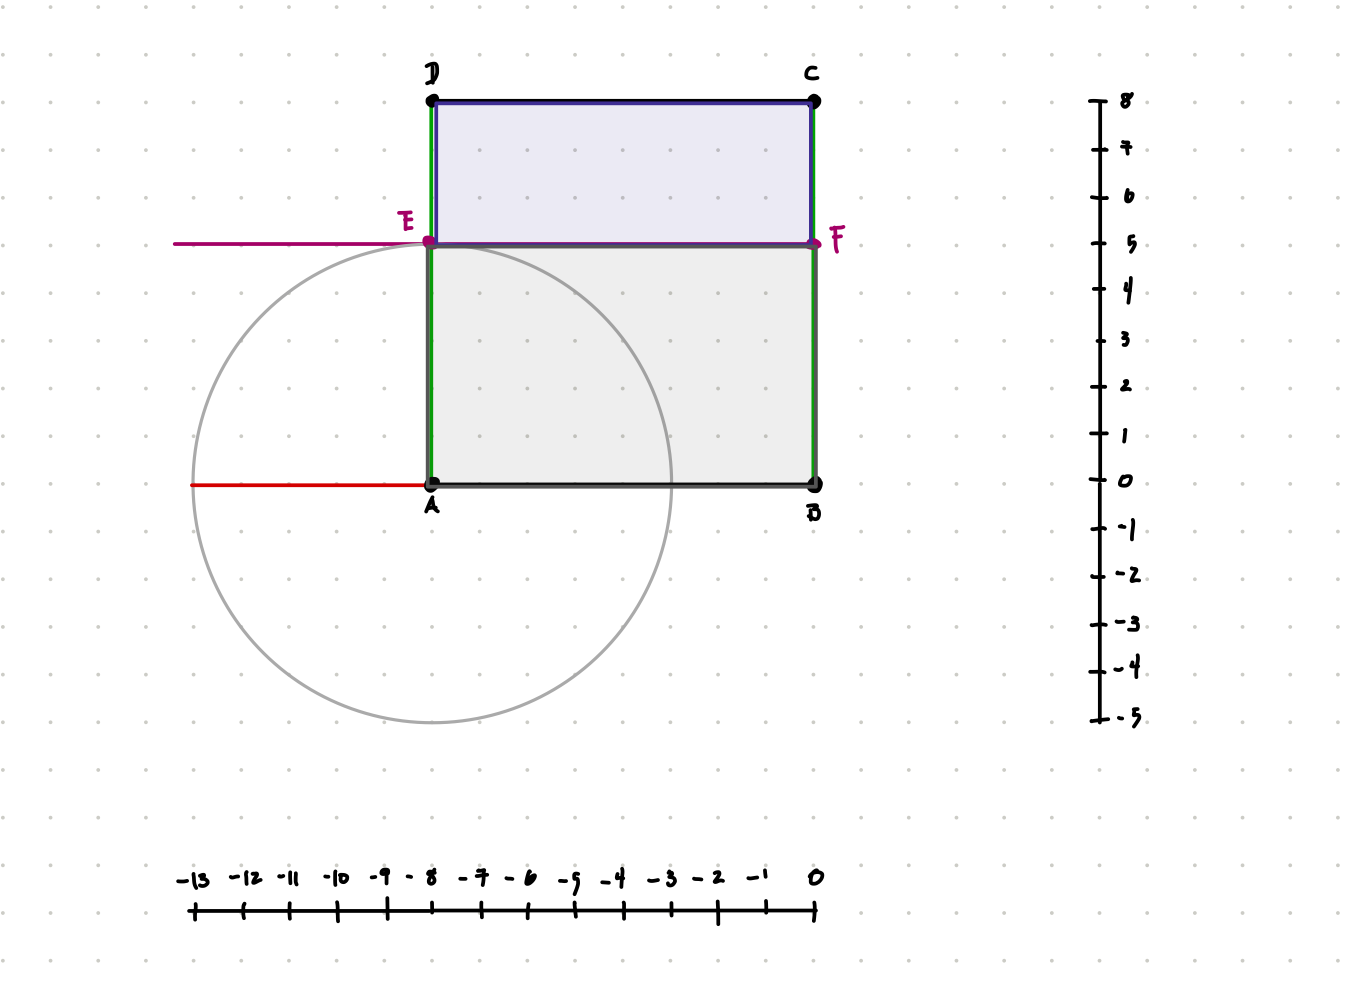
\includegraphics[width=8cm]{Capstone Presentation/Draft Diagrams/1.png}
    
    \caption{A base 8 regular rectangle dissected by a radius 5 circle.} 
    \label{Fig_Step_1}
\end{figure}

\begin{figure}[ht]
    \centering
    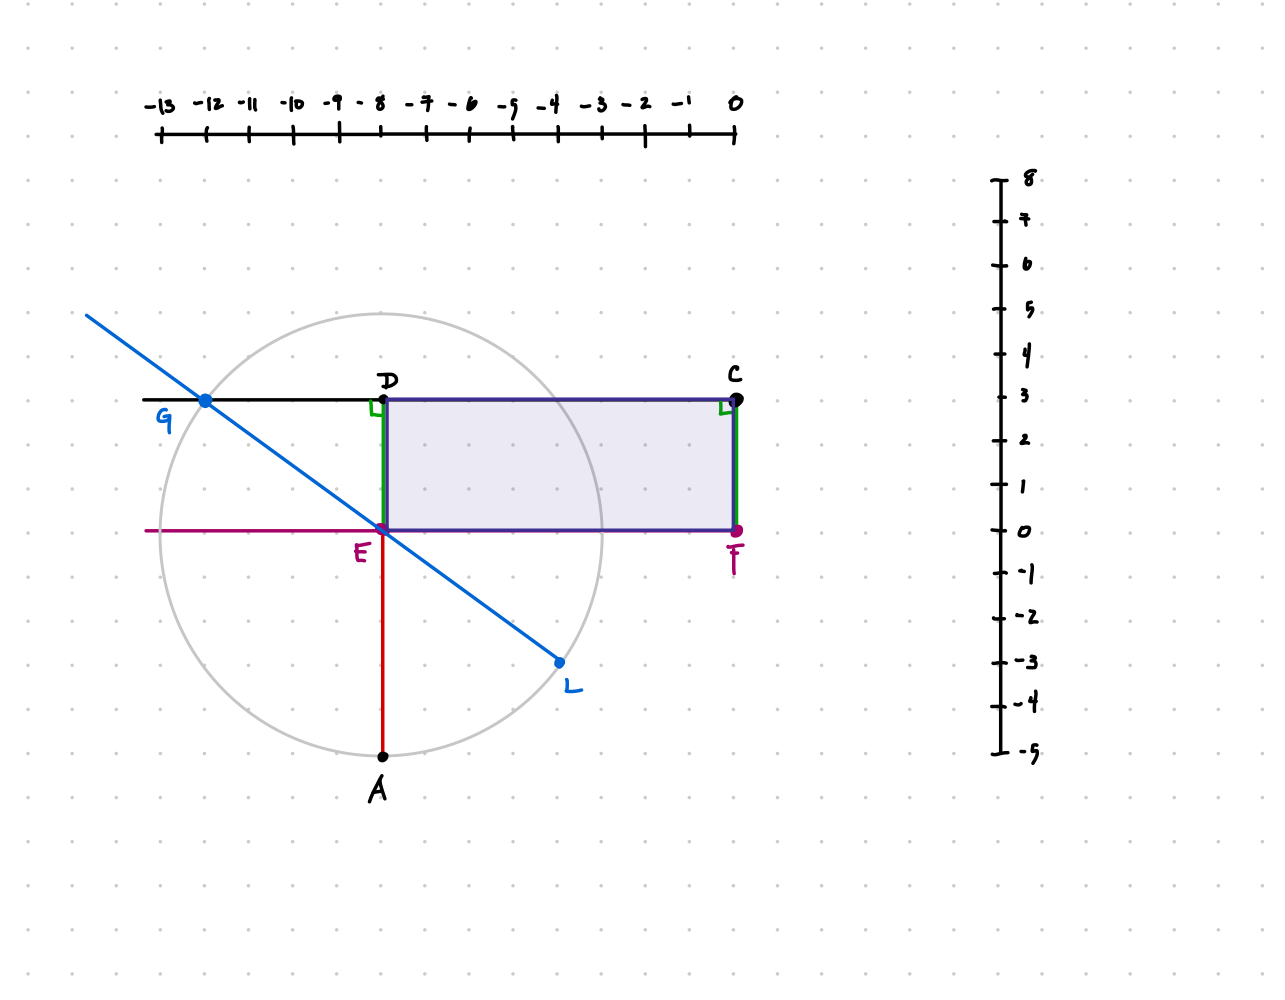
\includegraphics[width=8cm]{Capstone Presentation/Draft Diagrams/2.png}
    \caption{The line GL created using the diameter of the circle.}
     \label{Fig_Step_2}
\end{figure}

\begin{figure}[ht]
    \centering
    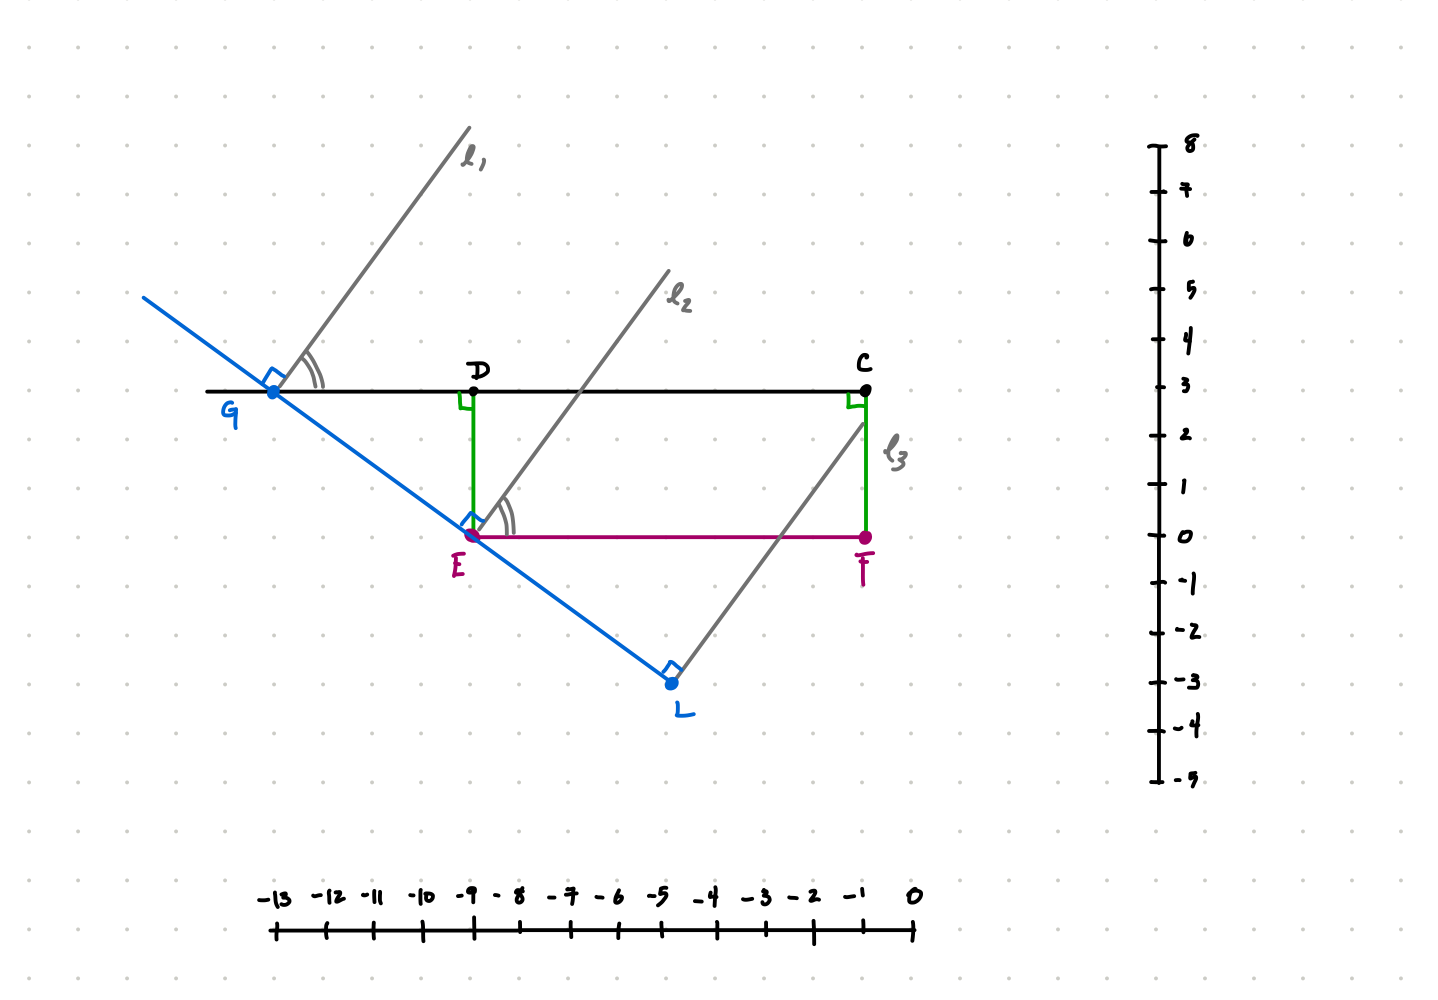
\includegraphics[width=8cm]{Capstone Presentation/Draft Diagrams/3.png}
    \caption{Three lines drawn perpendicular to line LG.}
     \label{Fig_Step_3}
\end{figure}

\begin{figure}[ht]
    \centering
    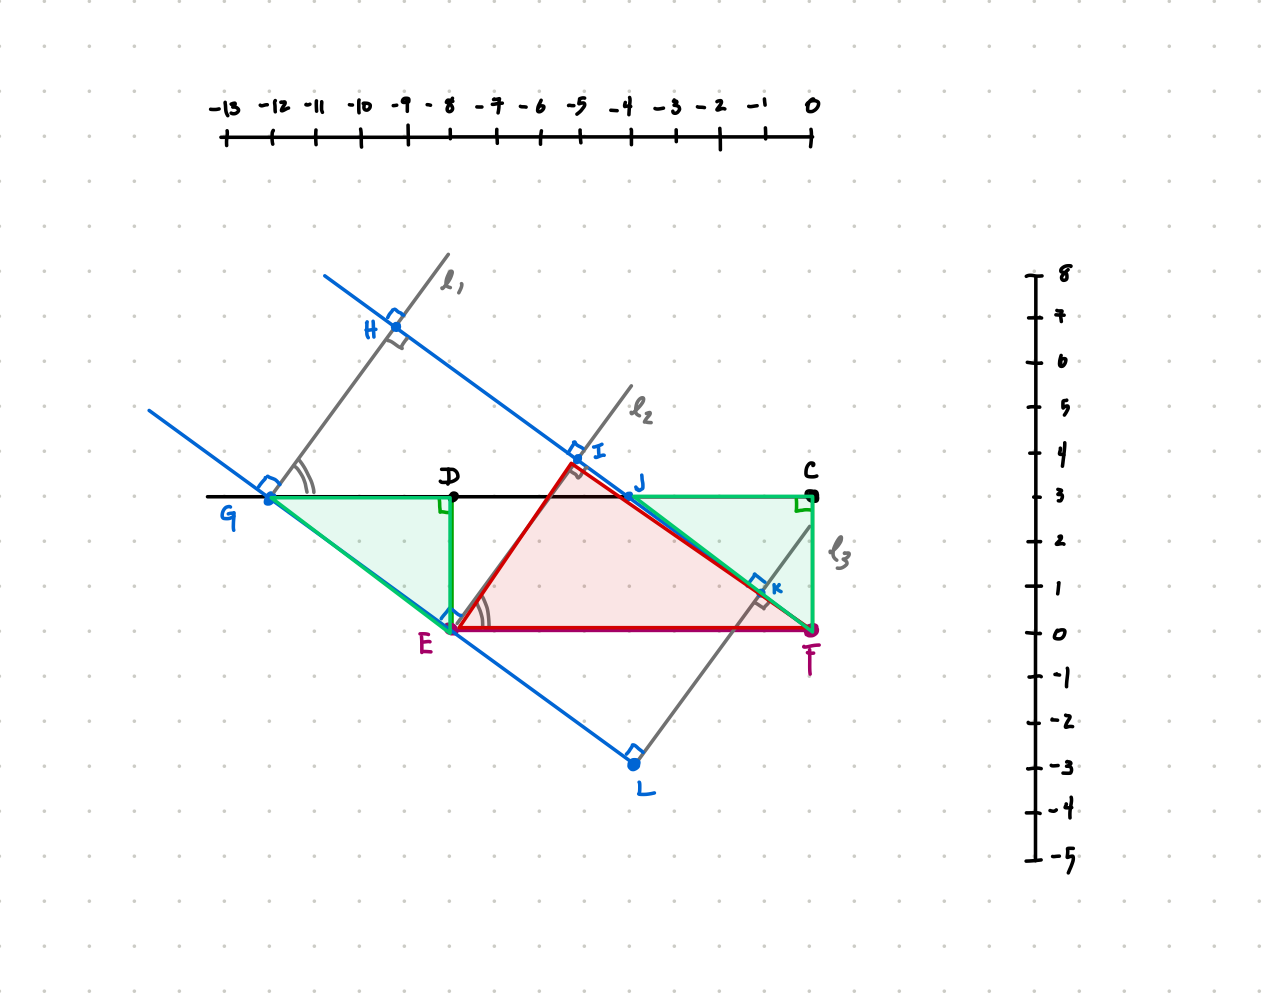
\includegraphics[width=8cm]{Capstone Presentation/Draft Diagrams/4.png}
    
    \caption{The red shaded triangle EIF and congruent green shaded triangles EDG and FCJ.}
    \label{Fig_Step_4}
\end{figure}

\begin{figure}[ht]
    \centering
    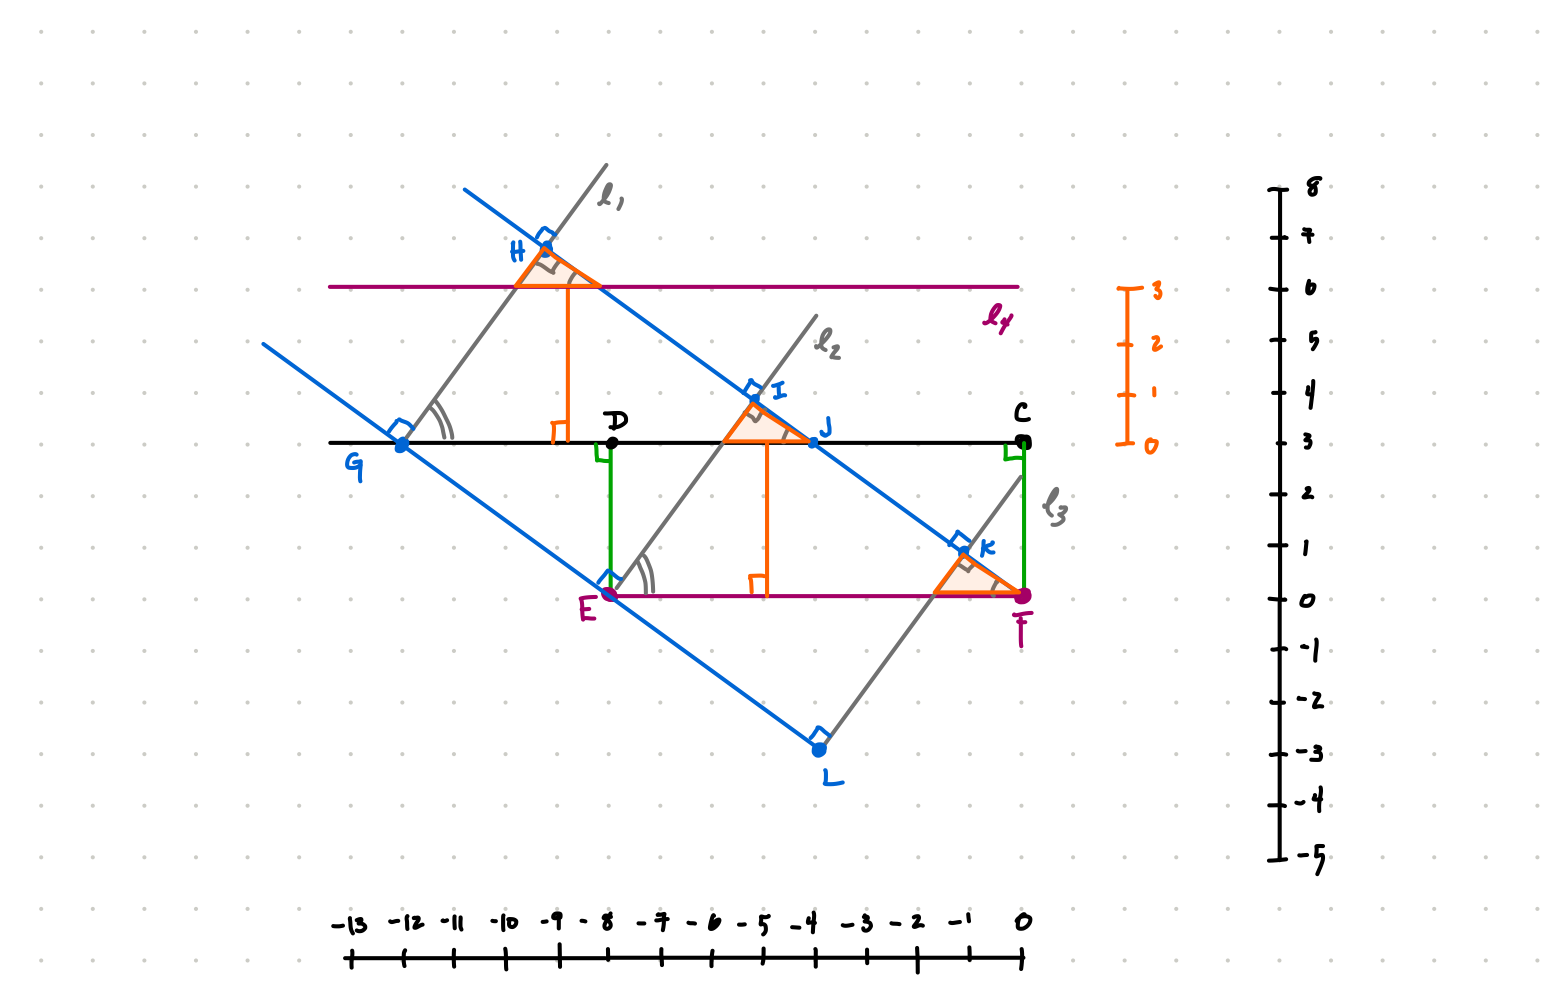
\includegraphics[width=8cm]{Capstone Presentation/Draft Diagrams/5.png}
    \caption{Three small orange shaded right triangles formed by a line L4 parallel to line CD drawn exactly 3 units from line CD.}
    \label{Fig_Step_5}
\end{figure}

\begin{figure}[ht]
    \centering
    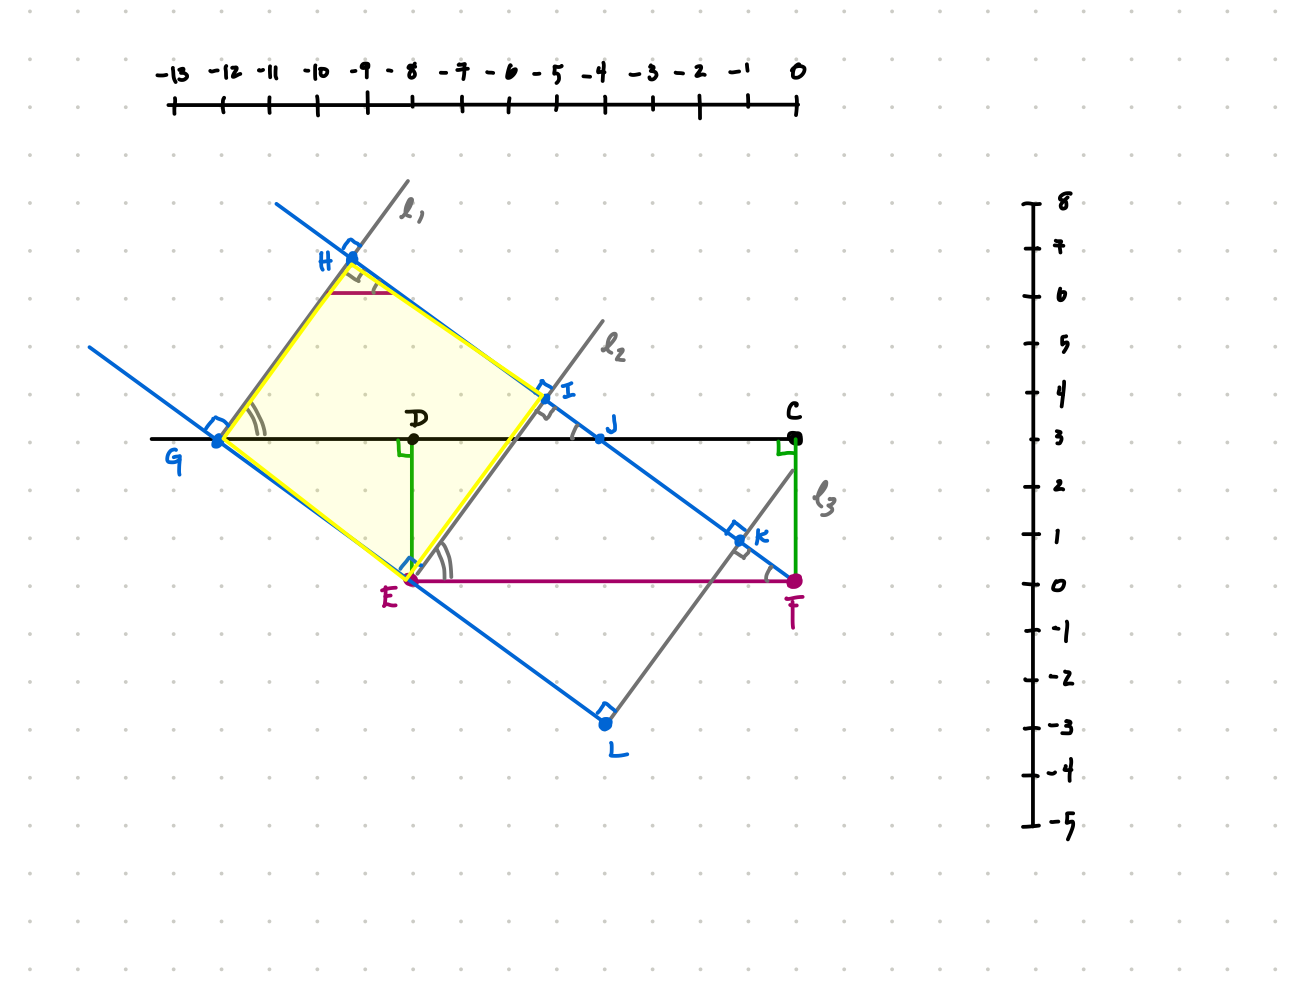
\includegraphics[width=8cm]{Capstone Presentation/Draft Diagrams/6.png}
    \caption{Two congruent rectangles EGHI, shaded in yellow, and EIKL which are composed of four pieces.}
    \label{Fig_Step_6}
\end{figure}

\begin{figure}[ht]
    \centering
    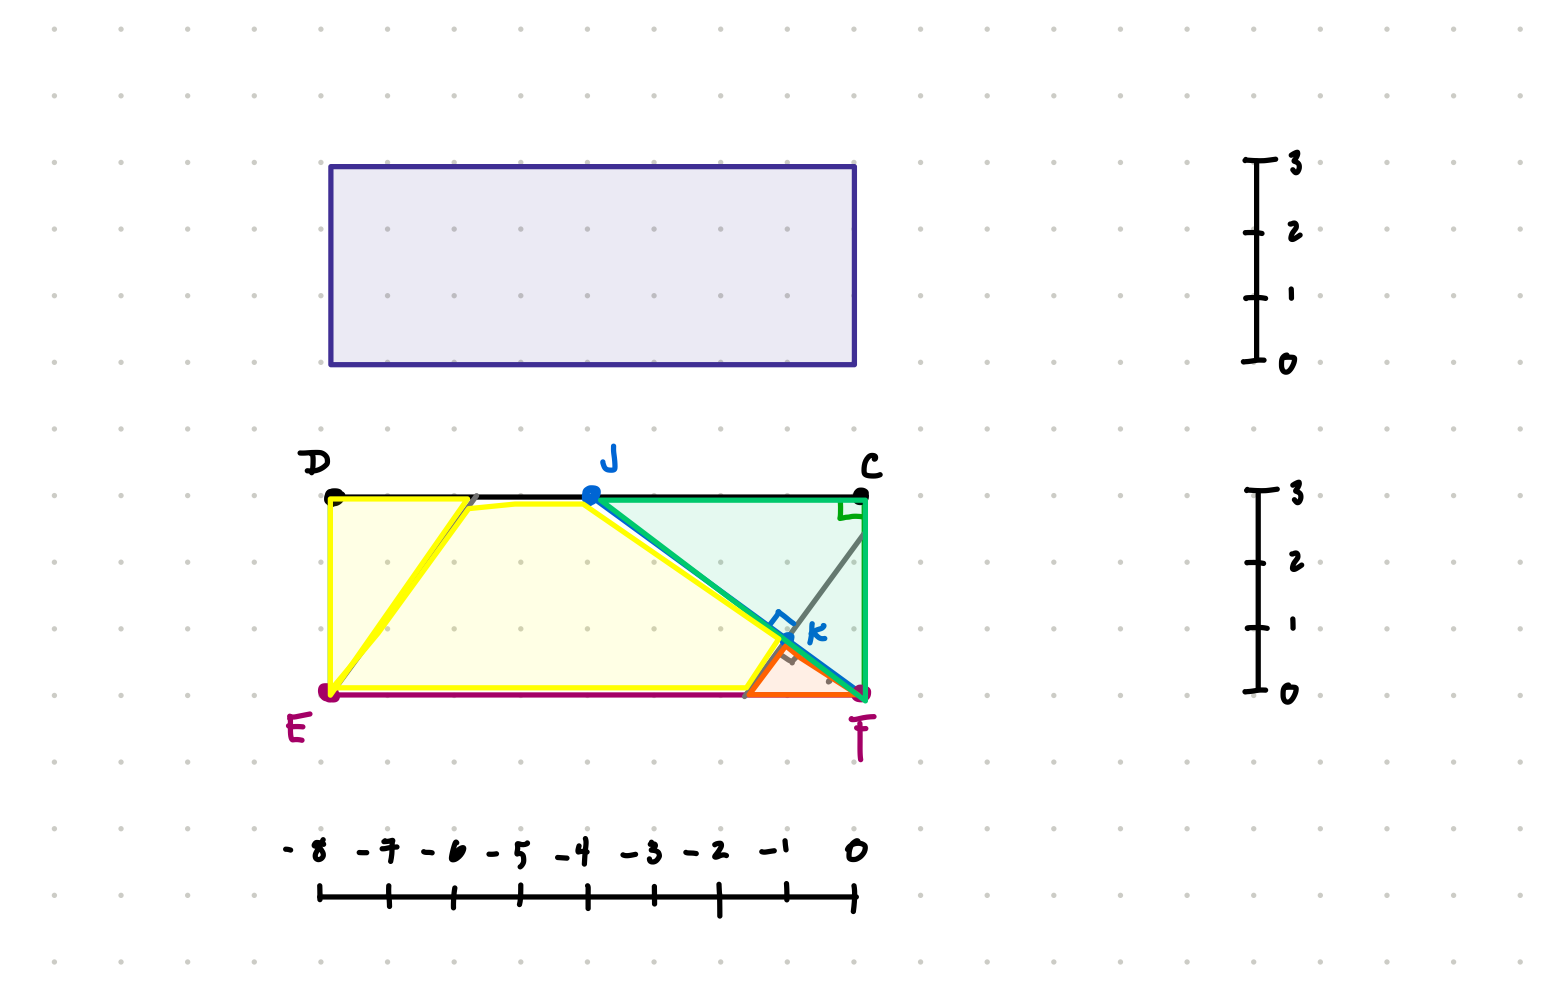
\includegraphics[width=8cm]{Capstone Presentation/Draft Diagrams/7.png}
    \caption{The original 8x3 portion of the 8x8 rectangle is shown here with the four pieces contained within.}
    \label{Fig_Step_7}
\end{figure}

\begin{figure}[ht]
    \centering
    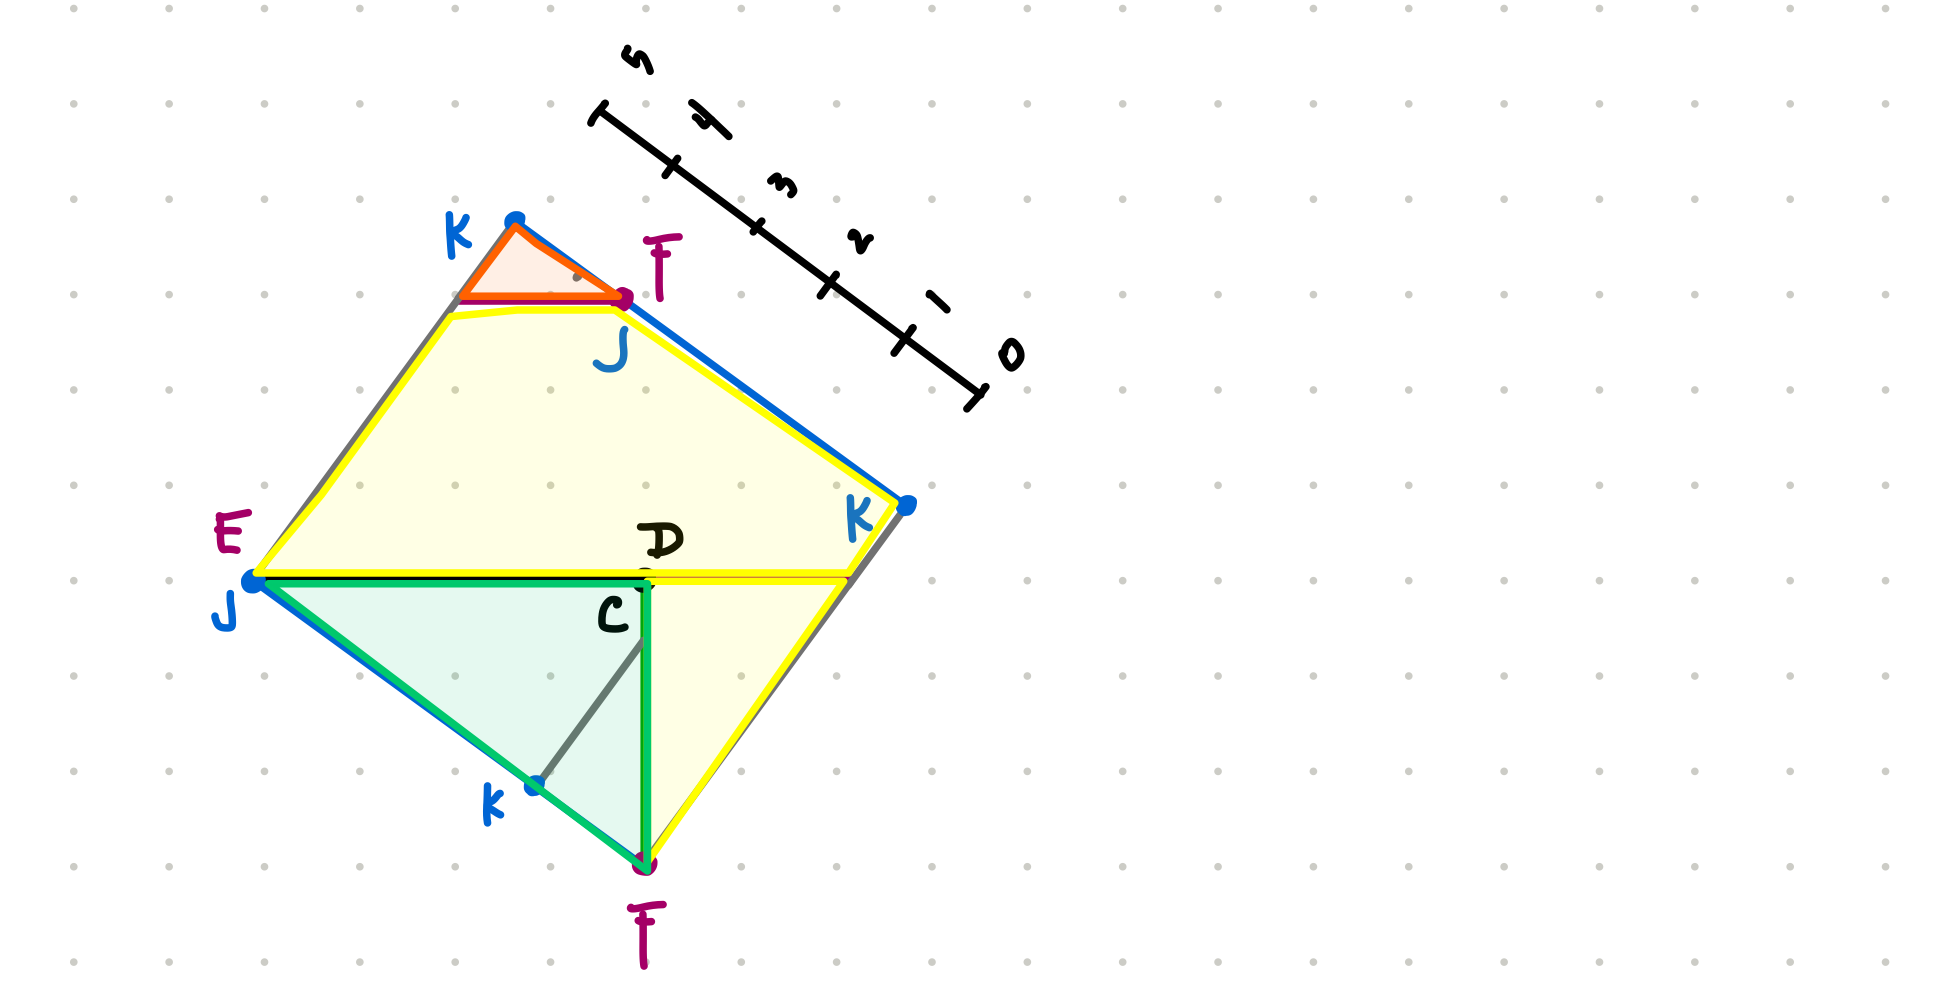
\includegraphics[width=8cm]{Capstone Presentation/Draft Diagrams/8.png}
    \caption{We can then rearrange the pieces to form our composed base 5 rectangle...}
    \label{Fig_Step_8}
\end{figure}

\begin{figure}[ht]
    \centering
    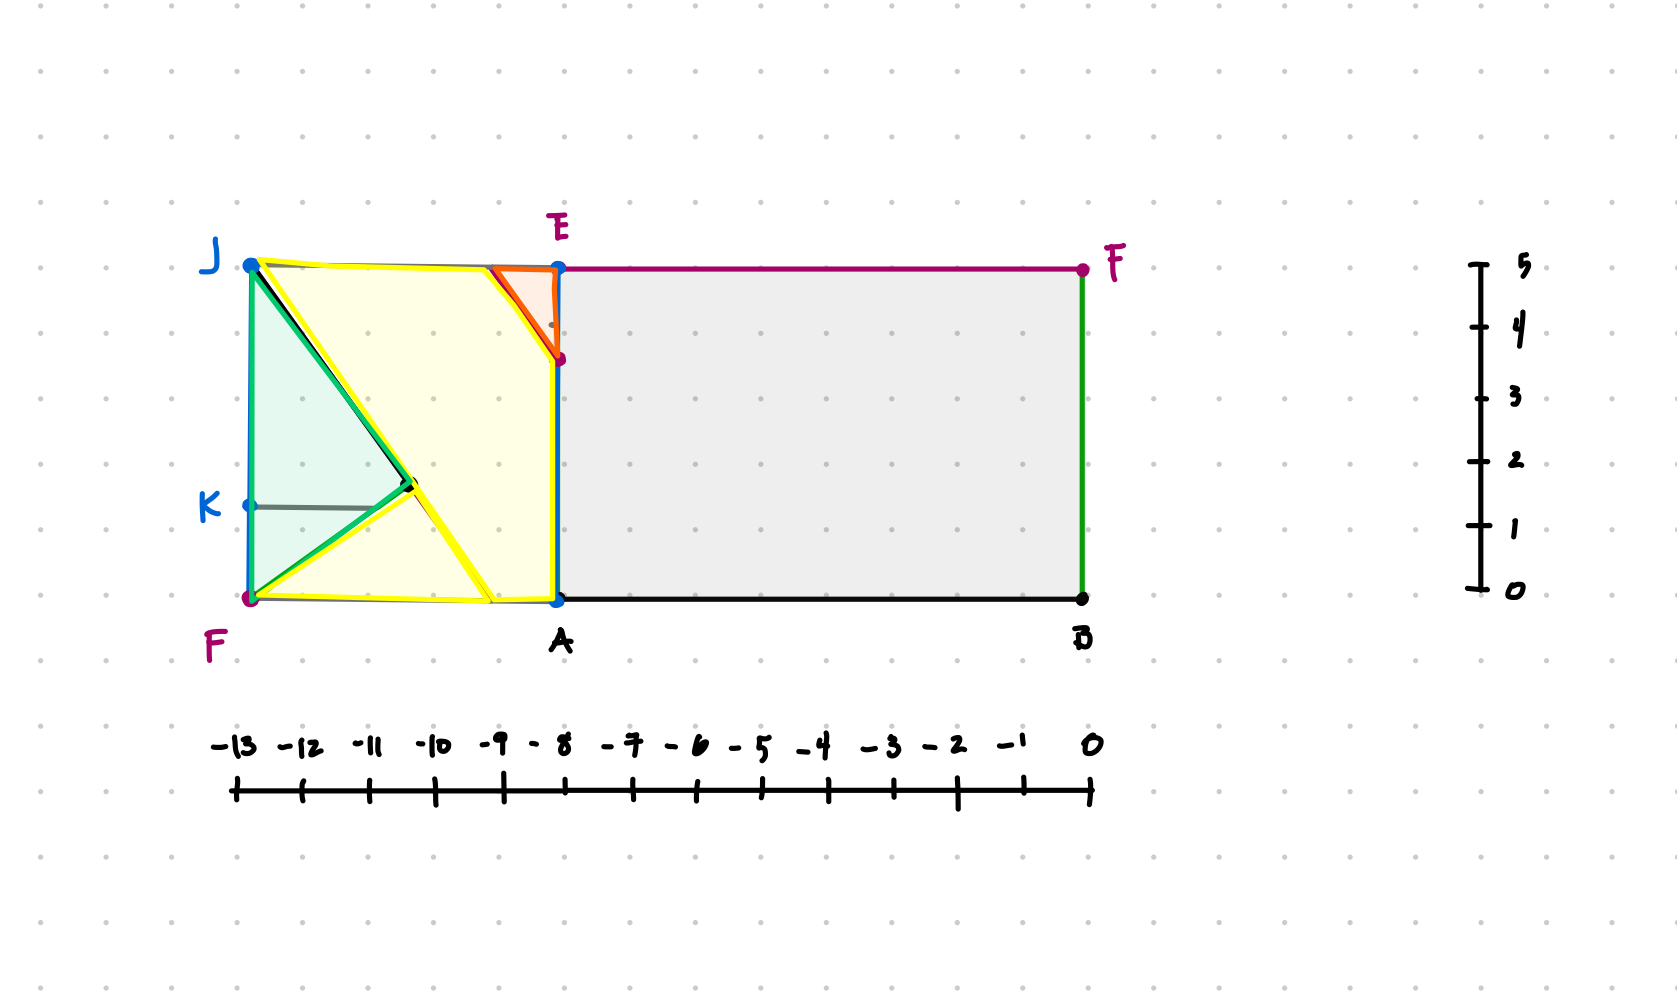
\includegraphics[width=8cm]{Capstone Presentation/Draft Diagrams/9.png}
    \caption{which can now be rotated and placed directly beside our 8x5 rectangle, thereby completing the problem.} 
    \label{Fig_Step_9}
\end{figure}


\FloatBarrier 

% - section{Equidecomposability, Part II}
\section{Equidecomposability, Part II}
Playing with more polygons (sans diagrams at the moment).

In this section, we show that any polygon can be transformed into any other polygon with the same area using the same rectangle with the same area between the two polygons. This transformation expands on the algorithm introduced and performed in Part I.

It can be demonstrated by taking a W (Figure \ref{Fig_Rough_1}) and turning it into a T and vice versa by using two identical rectangles that act as an intermediary between the two polygons, which are in this case, letters.

%This gets the point across well, but explaining about the rectangle and where it comes from/how it is used in the introduction might be helpful.%

\begin{enumerate}

    \item We will start with the W and draw non-intersecting lines that divide the entire polygon up into triangles (Figure \ref{Fig_Rough_2}).

    \item In the next step, we cut up the W into triangular pieces along the lines we just drew to divide our polygon (Figure \ref{Fig_Rough_3}).
    
    \item For each triangle, we use the hypotenuse, the longest edge, as the base of our rectangle and draw an orange line from the midpoint of one of the smaller edges to the midpoint of the last remaining edge (Figure \ref{Fig_Rough_4}).
    
    \item Drawing a blue line straight down from the apex of the triangle to the line connecting the midpoints of the smaller edges, we form two small right triangles (Figure \ref{Fig_Rough_5}).
    
    \item Cutting along both lines inside the triangle, we can, then, rotate them down from the edges midpoints (Figure \ref{Fig_Rough_6}).
    
    \item Recall that we do this for each triangle taken from the W.
    % - These two steps are redundant, but I'm not sure which sounds better, or whatnot.
    \item This rotation process forms many different sized rectangles out of all of the individual triangle pieces we have cut from the original W.
    
    \item At this point, we choose a base length of the mediating rectangle to transform all of the rectangle pieces we have just created into.
    % - This sentence sounds really wrong.
    
    \item Using the same algorithm we used in Part I, we decompose each rectangular piece to a rectangle with our chosen base length.
    
    \item Once we have constructed rectangles with identical bases from all of the pieces of the decomposed W, we can stack them up against each other at the bases that we have chosen in Step 2 to form one large rectangle that has the same area as the W that we started with.
    
    The dimensions of this rectangle will be used as an intermediary to both polygons.
    
    \item If we cut triangles out of the T that has the same area as the W using the same procedures, we can compose different rectangles that transform to rectangles that have the same base as those of the W.
    
    \item We can then form a large rectangle that has dimensions equivalent to the rectangle composed of the small rectangles from the W that will superimpose perfectly over it.
    
    \item Keeping all of the cuts from both rectangles, we can take all of the polygonal pieces formed by the superimposition of the rectangles and rearrange them to form either the polygon W or polygon T at will.
    
    Because the two intermediate rectangles share the same dimensions and are therefore equal in area, we can say that both polygons have the same area, and that we can decompose one to compose the other and vice versa.
    
    %These steps are very clear, and I am not sure what to change because I think they look great!%
    
\end{enumerate}

% - section{Equidecomposability, Part II} Diagrams
\begin{figure}[ht]
    \centering
    
\includegraphics[width=8cm]{Capstone Presentation/Draft Diagrams/Section 2 Diagrams/3.3 Rough Diagrams 1.png}
    
    \caption{The polygon W to be equidecomposed to a T.} 
    \label{Fig_Rough_1}
\end{figure}

\begin{figure}[ht]
    \centering
    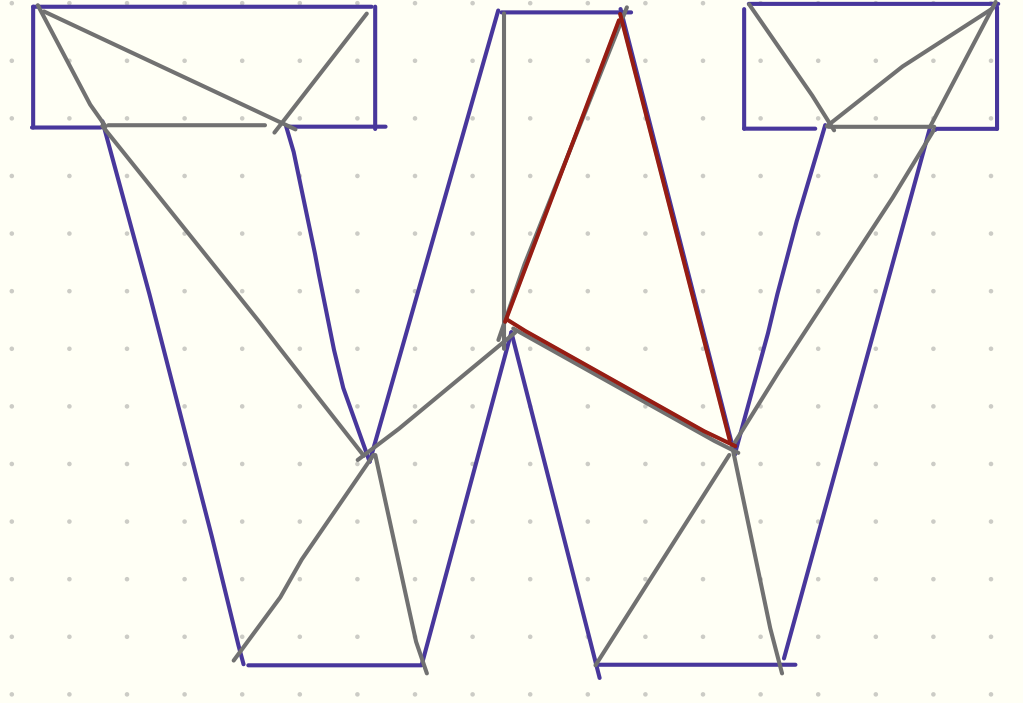
\includegraphics[width=8cm]{Capstone Presentation/Draft Diagrams/Section 2 Diagrams/3.3 Rough Diagrams 2.png}
    \caption{Non-intersecting lines forming triangles inscribed within the original W polygon.}
     \label{Fig_Rough_2}
\end{figure}

\begin{figure}[ht]
    \centering
    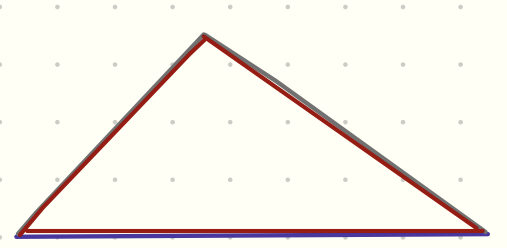
\includegraphics[width=8cm]{Capstone Presentation/Draft Diagrams/Section 2 Diagrams/3.3 Rough Diagrams 3.png}
    \caption{A triangle extracted and rotated from the original W polygon.}
     \label{Fig_Rough_3}
\end{figure}

\begin{figure}[ht]
    \centering
    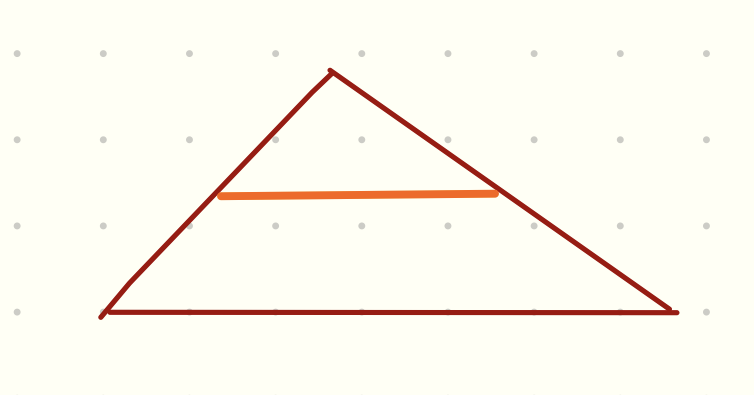
\includegraphics[width=10cm]{Capstone Presentation/Draft Diagrams/Section 2 Diagrams/3.3 Rough Diagrams 4.png}
    
    \caption{}
    \label{Fig_Rough_4}
\end{figure}

\begin{figure}[ht]
    \centering
    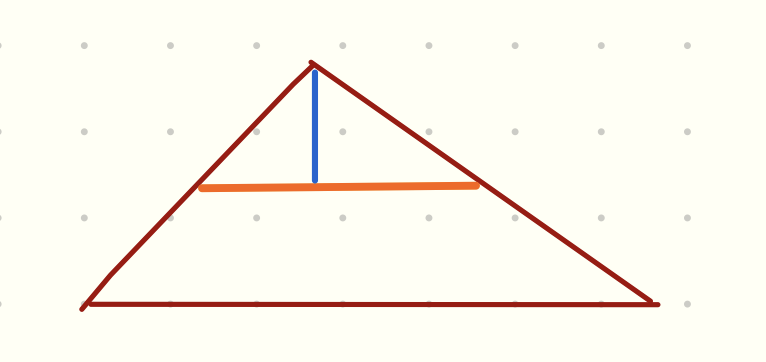
\includegraphics[width=10cm]{Capstone Presentation/Draft Diagrams/Section 2 Diagrams/3.3 Rough Diagrams 5.png}
    \caption{}
    \label{Fig_Rough_5}
\end{figure}

\begin{figure}[ht]
    \centering
    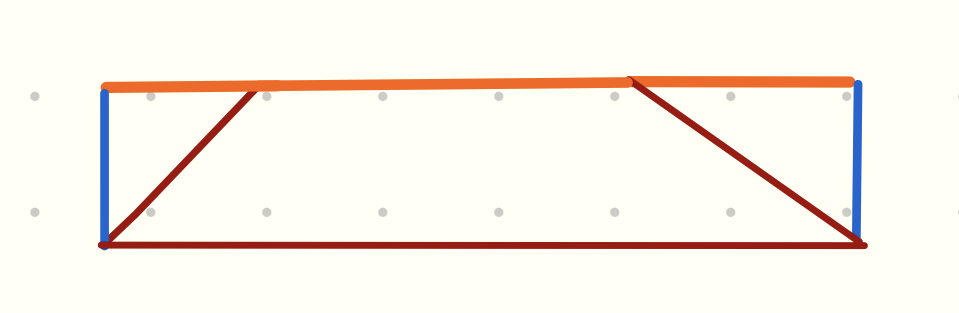
\includegraphics[width=8cm]{Capstone Presentation/Draft Diagrams/Section 2 Diagrams/3.3 Rough Diagrams 6.png}
    \caption{}
    \label{Fig_Rough_6}
\end{figure}

\begin{figure}[ht]
    \centering
    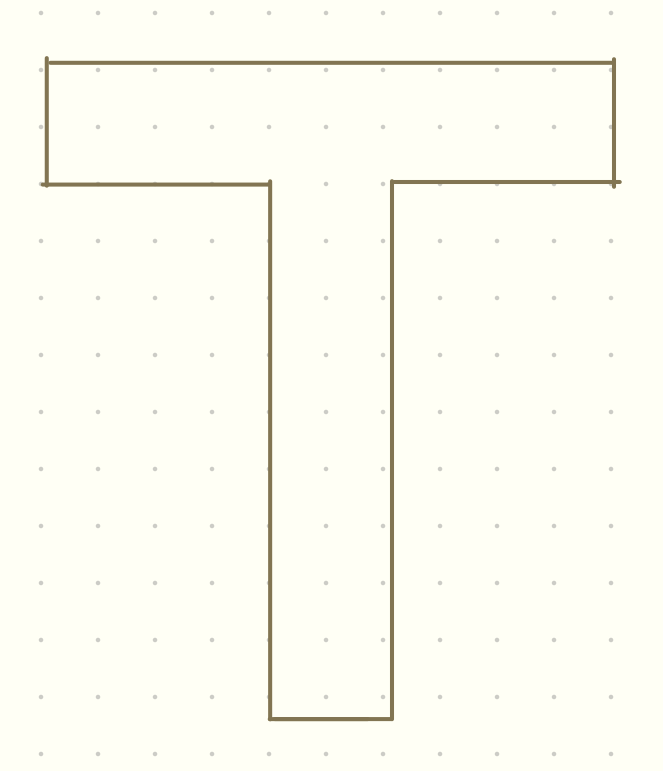
\includegraphics[width=8cm]{Capstone Presentation/Draft Diagrams/Section 2 Diagrams/3.3 Rough Diagrams 7.png}
    \caption{}
    \label{Fig_Rough_7}
\end{figure}

\begin{figure}[ht]
    \centering
    \includegraphics[width=8cm]{}
    \caption{}
    \label{Fig_Rough_8}
\end{figure}

\begin{figure}[ht]
    \centering
    \includegraphics[width=8cm]{}
    \caption{} 
    \label{Fig_Rough_9}
\end{figure}

\FloatBarrier

% - section{Equicomplementability}
\section{Equicomplementability}



% - section{Equicomplementability} Diagrams

\end{document}